\subsubsection{Sensoren}
In dem Block \textit{Sensoren} (Abbildung \ref{fig:sensoren}) sind alle Messeinheiten untergebracht. Die Idee dieses Blockes besteht darin, dass dieser adaptiv ist und somit leicht erweitert werden kann.\\

\begin{figure}[h]
	\centering
	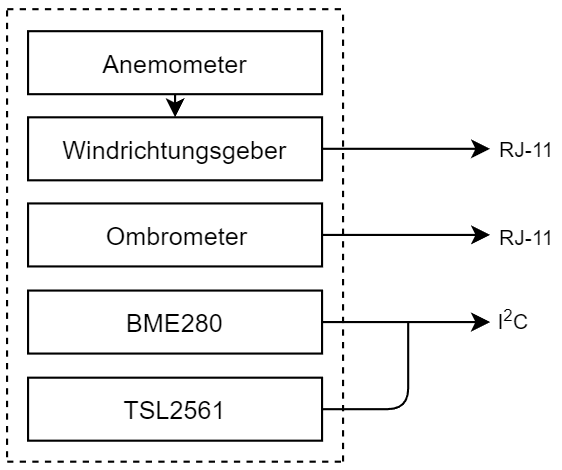
\includegraphics[width=0.5\textwidth]{graphics/Konzeptdiagramme/Sensoren.PNG} 
	\caption{Sensoren}
	\label{fig:sensoren}
\end{figure}

Der Lufttemperatur, -druck und -feuchtigkeits kombinierte Sensor BME280 und der Light-To-Digital Converter TSL2561 sind beide über das I$^2$C-Interface mit der \textit{MCU} verbunden. Das Anemometer kann direkt mit dem Windrichtungsgeber über die vorhandene RJ-11 Buchse angeschlossen werden, wobei dann der Ausgang des Windrichtungsgebers beide analogen Signale überträgt. Das Ombrometer wird separat angeschlossen.\\
